\section{Step Function}

A step function is a piecewise constant function as show in Figure \ref{fig:StepFunction}.

\begin{figure}[h]
\centering
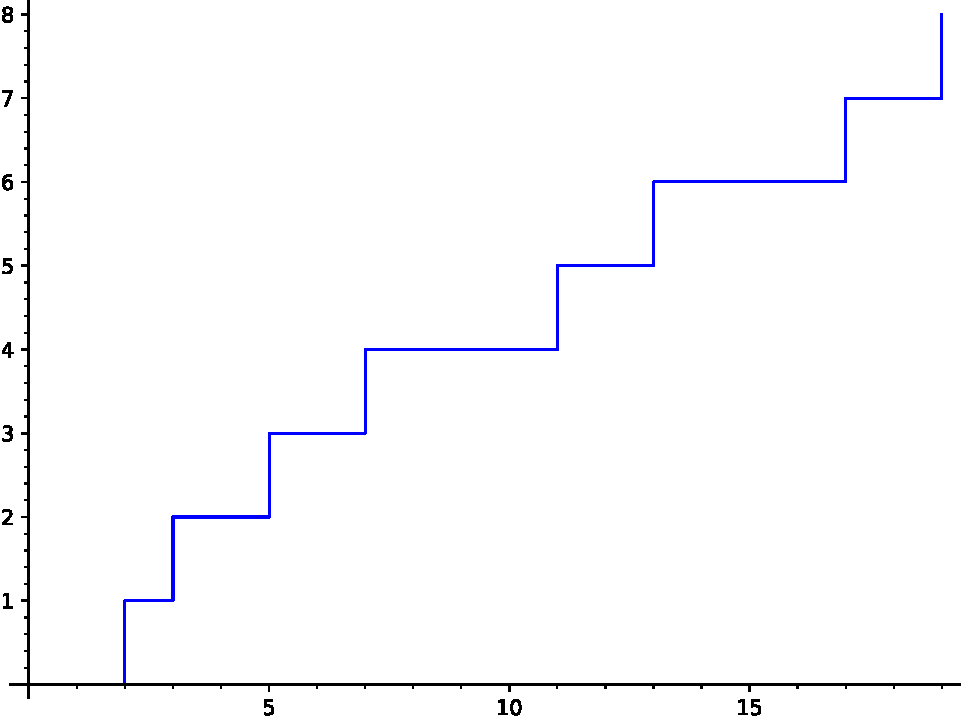
\includegraphics[width=8cm]{./figures/StepFunction.pdf}
\caption{Step function}
\label{fig:StepFunction}
\end{figure}

Mathematically,

$$
f(x) = 
\begin{cases}
\enspace c_0 & \text{ if } -\infty \le x < x_1, \\
\enspace c_1 & \text{ if } x_1 \le x < x_2, \\
\enspace \vdots & \qquad\quad\vdots \\
\enspace c_i & \text{ if } x_i \le x < x_{i+1}, \\
\enspace \vdots & \qquad\quad\vdots \\
\enspace c_n & \text{ if } x_n \le x < \infty,
\end{cases}
$$

A shopping mall is having its goods on sale. The discount rate varies and depends on the original marked price. The price discount table is as follows. For example, if an item has an original marked price of \$60, the sale price will have a $20\%$ off so you only need to pay \$48 for it.

\begin{center}
\begin{tabular}{l r } 
 \hline 
 Marked Price & Discount \\ [0.5ex] 
 \hline 
 $[0,10)$ & 5\% \\ [0.5ex] 

 $[10,30)$ & 10\% \\ [0.5ex] 

 $[30,50)$ & 15\% \\ [0.5ex]

 $[50,100)$ & 20\% \\ [0.5ex]

 $[100,200)$ & 30\% \\ [0.5ex]

 $[200,\infty)$ & 40\% \\
 \hline

\end{tabular}
\end{center}

\subsection{Implementation}
We write a function to compute the final price after discount for a given marked price. We propose two implementations.

\begin{minted}[samepage,frame=single,framesep=10pt,xleftmargin=10pt,linenos]{q}
// Implementation #1
.qe.math.finalPrice1:{[mp]
  prices:0 10 30 50 100 200;
  discounts:0.05 0.1 0.15 0.2 0.3 0.4;
  d:`s#prices!discounts;
  mp*1-d mp
  };
\end{minted}

Alternatively,
\begin{minted}[samepage,frame=single,framesep=10pt,xleftmargin=10pt,linenos]{q}
// Implementation #2
.qe.math.finalPrice2:{[mp]
  prices:0 10 30 50 100 200;
  discounts:0.05 0.1 0.15 0.2 0.3 0.4;
  mp*1-discounts prices bin mp
  };
\end{minted}

\subsection{Explanations}
In implementation \#1,

\begin{itemize}
\item Lines 3 and 4 define the price and discount lists
\item Line 5 creates a dictionary mapping from price thresholds to discount rate. Then a sorted attribute is applied to the keys of the dictionary. Setting a sorted attribute to a dictionary makes it a step function.
\item Line 6 first retrieve the discount rate for the given marked price and calculate the final price after discount.
\end{itemize}

In implementation \#2:

\begin{itemize}
\item Line 6 first finds the index of the price bucket where the marked price falls into and then retrieves the discount rate for the given marked price. It then calculates the final price after discount.
\end{itemize}

\subsection{Summary}

\begin{importantblock}
\textbf{Important Note}
\begin{itemize}
\item For a regular dictionary 
\begin{minted}{q}
d:10 20 30!0.1 0.2 0.3;
\end{minted}
\q{d[10]} gives $0.1$ but \q{d[11]} gives \q{0nf} since 11 is not a key of \q{d}.

\item For a dictionary with sorted attribute,
\begin{minted}{q}
d:`s#10 20 30!0.1 0.2 0.3;
\end{minted}
\q{d[10]} gives $0.1$ and \q{d[11]} also gives $0.1$ even though 11 is not a key of \q{d}. Because of the sorted attribute, \q{d} now is a step function and \q{d[x]} returns the value for the closest key which is smaller than \q{x}.
\end{itemize}
\end{importantblock}

\begin{noteblock}
\textbf{Knowledge Points}
\begin{itemize}
\item Set attribute: \href{https://code.kx.com/q/ref/set-attribute/}{x\#y}
\item Make a dictionary: \href{https://code.kx.com/q/ref/dict/#dict}{\q{x!y}}
\item Binary search: \href{https://code.kx.com/q/ref/bin/}{\q{bin}}
\end{itemize}
\end{noteblock}


\clearpage
